%% Copyright (C) 2023 by Jessica Scheick
%% v0.02 31May2023
%%
%% This work may be distributed and/or modified under the
%% conditions of the LaTeX Project Public License, either version 1.3
%% of this license or (at your option) any later version.
%% The latest version of this license is in
%%   http://www.latex-project.org/lppl.txt
%% and version 1.3 or later is part of all distributions of LaTeX
%% version 2005/12/01 or later.
%%
%% This work has the LPPL maintenance status `maintained'.
%% 
%% The Current Maintainer of this work is Jessica Scheick.
%% Please report problems to: jbscheick-at-gmail-dot-com
%%
%% This work consists of this file (ROSES-NASA-proposal_template.tex) and the associated class file (ROSES-NASA-proposal.cls)
%%
%% https://www.nasa.gov/wp-content/uploads/2023/09/2023-nasa-proposers-guide-final.pdf?emrc=7b5d89


%%%%%PREAMBLE%%%%%
\documentclass{ROSES-NASA-proposal}
\pagenumbering{roman}

\usepackage[margin=1in]{geometry}

\usepackage{pgfgantt}

\usepackage{minted}
\setminted[python]{
  frame=lines,
  bgcolor=LightGray,
}
\setminted[bash]{
  frame=lines,
  bgcolor=LightGray,
}

\usepackage{enumitem}

\usepackage{xcolor} % to access the named colour LightGray
\definecolor{LightGray}{gray}{0.97}

\usepackage[
    colorlinks=true,
    urlcolor=black,
    linkcolor=black,
    citecolor=black
]{hyperref}


% https://www.overleaf.com/latex/examples/simple-stylish-box-design/stzmmcshxdng
\usepackage[many]{tcolorbox}    	% for COLORED BOXES (ti
\definecolor{sub}{HTML}{cde4ff}     % setting sub color to be used
\newtcolorbox{boxC}{
    colback = sub, % background color
    boxrule = 0pt  % no borders
}


\usepackage{listings}
\definecolor{codegreen}{rgb}{0,0.6,0}
\definecolor{codegray}{rgb}{0.5,0.5,0.5}
\definecolor{codepurple}{rgb}{0.58,0,0.82}
\definecolor{backcolour}{rgb}{0.95,0.95,0.92}

\usepackage{natbib}
\bibliographystyle{agufull08}
% use \citep and \citet to cite articles

\usepackage{xspace}
\newcommand{\earthaccess}{\textit{earthaccess}\xspace} % always use this instead of spelling out "earthaccess"!
\renewcommand\bibsection{\section{\refname}} % use this to add a section number to the references

%%%%%DOCUMENT START%%%%%
\date{}

%variable declaration to include NSPIRES entered cover info in compiled pdf or not
%be sure to compile multiple times before submitting and check table of contents page numbers
\newif\ifsubmitpdf
\submitpdffalse  
%submitpdftrue

\begin{document}

%%%%%PROPOSAL INFORMATION ENTERED DIRECTLY INTO NSPIRES%%%%%
\ifsubmitpdf
\else
\begin{center}
{\LARGE\MakeUppercase {Notes and Information}}
\end{center}

\noindent {\large \textbf{Title:} Elevating \earthaccess: Cultivating an Ecosystem of People and Tools to Streamline NASA Earthdata Workflows}

\noindent \textbf{Investigators + Titles:} Walt Meier (PI), Luis López Espinosa (Co-I), Matt Fisher (Co-I), Amy Steiker (Co-I), Andrew P. Barrett (Co-I), Joseph H. Kennedy (Co-PI), Jessica Scheick (Co-PI)


\section*{Project Summary} \label{summary}
4000 character max (including spaces) summary of the proposed project here.
%4000 character max (including spaces) for proposal abstract/project summary

NASA Earth science data, along with data from other national and international scientific agencies, are moving their data holdings to the the commercial cloud, allowing large-scale, cloud-based workflows.  However, the Earth science community has faced a steep learning curve in transitioning from local computing environments to the cloud and in adapting to disparate tools and services.  Data access requires programmatic interfaces with the Common Metadata Repository (CMR) and Earthdata Login (EDL). The complexity of using low-level Python tools to access these tools is sometimes an insurmountable hurdle to the work researchers want to accomplish.  The \earthaccess library grew out of the need for an easy-to-use programmatic interface to search for and access NASA data.  It now provides a unified approach to searching for and accessing data whether users are working on a local machine or in the cloud. The library is under active development and continues to gain popularity.  To sustain this growth we need to streamline maintenance and development, lower barriers for new contributors to participate, and add new features to simplify usability further and enable future development.

We seek to create the community and software frameworks needed to sustain community development of \earthaccess, thereby enhancing reproducible and streamlined data discovery and access patterns across the NASA Earth Sciences Division. We have three main objectives to to accomplish this goal. 
 \textbf{We will strengthen community engagement in \earthaccess by reducing the barriers to participation in the project for software engineers and non-engineers alike}.  This will be achieved by building documentation and tools to help community members contribute and by cultivating a community through community calls, blogs, hackweeks, tutorials, and workshops.  

\textbf{We will improve software sustainability and lower the maintenance burden}.  A key part of this is minimizing the technical knowledge required to contribute to the project by simplifying creating issues and feature requests, setting up development environments and formatting code contributions. Automating the busy-work of managing contributions by taking advantage of GitHub actions and streamlining the tasks of packaging, distribution and testing of the library will remove a considerable burden from maintainers, enabling more and richer human interactions.

\textbf{We will implement software features to make \earthaccess more widely usable and easily customizable so that we can embrace the diversity of NASA data and user needs}.  Our aim is that \earthaccess can power open-source science.  A fundamental aspect of this is reproducibility.  We will build functionality to allow users to save and reproduce \earthaccess search parameters and results.  A command line interface will enable non-Python users to use \earthaccess.  We will create a plugin interface that will allow easy extension of \earthaccess and integration with tools and services such as NASA Harmony, the Alaska Satellite Facility's Hybrid Pluggable Processing Pipeline (HyP3), and \textit{icepyx}.
    
Effective use of NASA's increasingly large data volumes to answer pressing research and societal questions critically depends on users' ability to access and use those data. \earthaccess already provides a set of tools for easily discovering and accessing those data and is poised to take that utility to the next level. Our proposed tasks provide a broader set of tools that build on our strong foundation.

%%%%%PROPOSAL TEXT NOT ENTERED THROUGH NSPIRES%%%%%
\newpage

\ifsubmitpdf
\else
\begin{center}
{\LARGE\MakeUppercase {Scientific/Technical/Management Plan}}
\end{center}
\fi

\tableofcontents

\newpage 
%%%%%Science/Technical/Management Plan%%%%%


\section{Introduction}
\pagenumbering{arabic}

By 2026, most, if not all, of NASA Earth science data will be stored in the commercial cloud. Other national and international scientific agencies are also moving their data to the cloud (e.g., both USGS's Landsat and ESA's Sentinel-2 data are available in Amazon Web Services (AWS) cloud storage). This data migration presents tremendous opportunities and challenges for the Earth science community. Extensible cloud-based computing close to cloud-hosted data enables large-scale computing on a rapidly growing volume of data without the need to download this data to a local machine. The time ``to science'' -- actually doing data analysis instead of data wrangling -- can be significantly reduced. However, researchers face a steep learning curve when moving from familiar \textit{download and analyze} workflows on laptops and local workstations to cloud-based \textit{analysis in place} workflows in often-unfamiliar cloud environments. A key challenge encountered early on in cloud-based workflows is learning how to search for and access data. Web-based graphical user interface (GUI) applications for data search and access, such as NASA Earthdata Search, cannot be used directly in cloud environments. Moreover, point-and-click interfaces do not facilitate reproducible workflows such as saving searches and access patterns that can be rerun by researchers' own \textit{future selves} \citep{lowndes_better_path_2017} or by other researchers who want to reproduce, repeat, or update analyses.

The \earthaccess Python library grew out of teaching programmatic and cloud-based data search and access workflows at the University of Washington (UW) eScience Institute's ICESat-2 Hackweeks and the NASA Openscapes Science Champions program. Through these experiences, it became apparent that researchers needed an easy-to-use programmatic interface that abstracts the underlying NASA and AWS authentication and search components needed for these workflows. Users were required to know and interact with many different systems programmatically, including: NASA Earthdata Login (EDL) for access to NASA data; AWS credentials for accessing AWS data storage; AWS Simple Storage Service (S3) for interacting with cloud data storage; and the NASA Common Metadata Repository (CMR) for discovering and accessing NASA Earth science data and associated services. Pre-existing low-level Python libraries used to interact with these systems proved confusing, error-prone, and time-consuming for researchers unfamiliar with programmatic data access. This creates multiple barriers to achieving what researchers ultimately wanted to accomplish: data analysis and doing science.

\earthaccess allows users to search for and access NASA Earth science data using as few as three Python statements instead of the tens to hundreds of lines of code that are required when using lower-level Python libraries such as \textit{requests}. The library is an intuitive and unified set of functions that are agnostic about the operating system and where data are stored. Researchers can use the same code to log in, search for, and access data whether they are working locally on their laptop, on a High Performance Computing (HPC) node, or on a cloud-hosted compute instance. The library is designed to interface seamlessly with standard tooling across the Python Earth science ecosystem, including Xarray \citep{hoyer2017xarray}, Dask \citep{rocklin2015dask}, Pandas \citep{reback2020pandas, pandas-mckinney}, and Geopandas \citep{geopandas}. Workflows using \earthaccess can be presented simply and clearly, and easily shared in Jupyter Notebooks \citealp{JupyterNotebook} or Python scripts, facilitating reproducible and repeatable science.
%\vspace{8pt}


\subsection{Objectives}

The development of \earthaccess and its community of contributors and users has grown organically, cultivated so far through varying levels of engagement by DAACs and scientific community volunteers. As we support and onboard an increasing number of end-users and community members, this current model will be challenging to sustain with existing resources. In order to continue to grow, innovate new ways to reduce time to science, and support our community, additional support is needed.

\textbf{We seek to create the community and software frameworks needed to enable and sustain community development of \earthaccess, thereby enhancing reproducible and streamlined data discovery and access patterns across the NASA Earth Sciences Division. We aim to accomplish this through specific maintenance, development, and community activities:} 

\begin{enumerate}
    \item Strengthen the community engagement of \earthaccess to lower participation barriers for software engineers and non-engineers alike (Section \ref{community}).

    \begin{itemize}[itemsep=-.1em]
        \item Build documentation and tools for new contributors.
        \item Build community through education and outreach.
    \end{itemize}
    
    \item Improve software sustainability and lower the maintenance burden (Section \ref{maintain}).

    \begin{itemize}[itemsep=-.1em]
        \item Remove or lower barriers to contributing by minimizing the required technical knowledge.
        \item Automate the busy-work of management of contributions to enable more human interaction.
        \item Streamline packaging, distribution and testing.
    \end{itemize}
    
    \item Implement software features to make \earthaccess more widely usable and customizable to embrace the diversity of NASA data and user needs (Section \ref{features}).

    \begin{itemize}[itemsep=-.1em]
        \item Provide reproducible searches allowing users to save \earthaccess search options and results for use later.
        \item Build a Command Line Interface (CLI) to enable non-Python users to use \earthaccess.
        \item Implement a plugin interface to support extended functionality and integration with other tools and services, including NASA Harmony, the Alaska Satellite Facility's Hybrid Pluggable Processing Pipeline (HyP3), and \textit{icepyx}.
    \end{itemize}

\end{enumerate}


Our team has extensive experience in the open-source software space and detailed technical knowledge of NASA data center infrastructure and datasets. It includes scientific data users from multiple disciplines, research software engineers, and community managers with experience in a wide range of data access and use patterns. Many of our team members are maintainers of \earthaccess, and all are core contributors as well as users. We collectively maintain and contribute to tens of libraries in the open source space and have helped organize and administer a similar number of workshops and tutorials. However, the current level of support for \earthaccess is vastly outpaced by its growth, requiring additional supported team members.

The success of this project will ultimately be measured by adoption across the Earth Science Division and ease of data user transition to cloud-based workflows. Effective use of NASA's increasingly large data volumes to answer pressing research and societal questions critically depends on users' ability to access and use those data. \earthaccess already provides a set of tools for easily discovering and accessing those data and is poised to take that utility to the next level. Our proposed tasks provide a broader set of tools that build on our strong foundation.


\subsection{History and impact of \earthaccess} \label{history}

\earthaccess was initially released in alpha as “earthdata” on 21 September, 2021. Leading up to the 2022 AGU Fall Meeting, the library proceeded to a beta release, followed by its first formal release available in both PyPI and Conda Forge along with the renaming to ``\earthaccess''. As of June 2024, \earthaccess is at its 20th release, Version 0.9.0. Its public NSIDC GitHub repository, under an MIT License, contains rich conversation and feature requests through its hundreds of open issues and discussions. The library is growing quickly and continues to gain popularity. As of June 2024, \earthaccess has seen over 31,000 downloads via Conda \footnote{\url{https://anaconda.org/conda-forge/earthdata} and \url{https://anaconda.org/conda-forge/earthaccess} accessed 2024-06-04. \earthaccess was formerly called \textit{earthdata}, so the totals are combined.}, over 3,500 monthly downloads from PyPI \footnote{\url{https://pypistats.org/packages/earthaccess} accessed 2024-06-04.}, and 365 stars on \href{https://github.com/nsidc/earthaccess}{GitHub}. \earthaccess is also used as a dependency \footnote{\url{https://github.com/nsidc/earthaccess/network/dependents} accessed 2024-06-04.} by at least ten commonly-used Python geospatial packages including \textit{icepyx}, \textit{its\_live}, \textit{leafmap}, and \textit{prefect-earthdata}. Libraries and projects such as \textit{leafmap}, \textit{icepyx}, Coiled, and \textit{SlideRule} are collaborating with the \earthaccess community directly to avoid duplication of effort. \earthaccess is also used on hosted cloud platforms like those provided by NASA VEDA, Openscapes, CryoCloud and the Pangeo project (Figure \ref{fig:earthaccess-ecosystem}).

\begin{figure}[h]
    \centering
    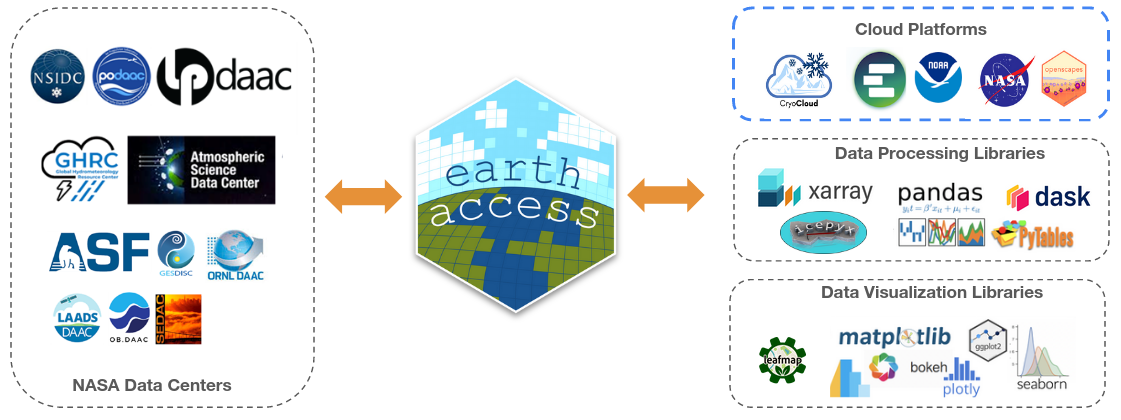
\includegraphics[width=0.95\linewidth]{images/ecosystem.png}
    \caption{The \earthaccess ecosystem supports data distributed by NASA DAACs and integrates with several open-source geospatial libraries and cloud platforms. }
    \label{fig:earthaccess-ecosystem}
\end{figure}

\earthaccess gained adoption by scientists and other DAAC teams through NASA Openscapes, a group of DAAC mentors supporting Earth science researchers to migrate their scientific analysis workflows to the cloud. \earthaccess is also the primary tool taught within the Python and R lessons of the NASA Openscapes Earthdata Cloud Cookbook. Multiple DAACs, including National Snow and Ice Data Center (NSIDC) DAAC, Alaska Satellite Facility (ASF) DAAC, Physical Oceanography DAAC (PO.DAAC) and Land Processes (LP) DAAC, continue to replace their existing Python guidance, which depends on multiple lower level libraries and can be challenging to reproduce across systems, in favor of \earthaccess to teach simplified discovery and access workflows (Listing \ref{listing:1}).

\begin{listing}[H]
\begin{minted}{python}
import earthaccess
import xarray as xr

earthaccess.login()

results = earthaccess.search_data(
    doi="10.5067/SLREF-CDRV3",
    bounding_box=(-10, 20, 10, 50),
    temporal=("1999-02", "2019-03"),
    count=10
)

ds = xr.open_mfdataset(earthaccess.open(results))
\end{minted}
\caption{Three Python statements to get NASA MEaSUREs Sea Surface Height data as an \textit{xarray} data cube.}
\label{listing:1}
\end{listing}


\subsection{\earthaccess project management: A model for NASA's community driven development}

\earthaccess is a \textit{community-owned} open-source project, exceeding the requirements for open-source software in NASA SPD41A \citep{SPD41A}. This way of working is not a new construct; it happens in an open, collaborative environment where the community and users contribute to and benefit from it in equal terms. On the \earthaccess project, you don't have to be a DAAC software engineer to participate. The community spans a range of backgrounds and Python coding experience, including affiliations with NASA DAACs, educational institutions, and private industry, united with a common vision to streamline Python-based NASA Earth science data access. 

In community-owned open-source software, there is no “definition of done”; instead, development evolves in response to the community and their needs \citep{eghbal_working_2020}. In many major open-source projects (e.g. numpy, GDAL, Project Jupyter) there are no stakeholders or closed executive boards. Instead, over years of impact, these projects have established open governance models with steering councils and institutional partners. Project Jupyter, an open source project that created Jupyter Notebooks, has an Executive Council responsible for overall management of the project and a Software Steering Council that oversees software development \footnote{See \url{https://jupyter.org/about}}. In projects more similar to \earthaccess in size and scope, projects are managed by a few core maintainers with an engaged community of users and contributors working together. One example is \textit{Xarray}, which has a team of 24 core maintainers and over 370 contributors \footnote{See \url{https://xarray.dev/team}}.

The early success of \earthaccess came from the project's ability to evolve quickly in response to user needs. This approach allows software reuse. Developers or researchers may see that \earthaccess does 80\% of what they want and request or, even better, contribute a new feature to achieve the remaining 20\%. The alternative may involve reinventing the wheel, wasting valuable time that could have been spent doing science. This breaking down of silos and facilitating direct communication between NASA software engineers and Earth science researchers is what sets \earthaccess apart from other open-source NASA tools.  In the course of the proposed work, we expect to learn more about the community development and adapt our approach in response to new challenges. But we anticipate that this community development framework employed by \earthaccess can serve as a model for other NASA Earth Science Division projects. 

\subsection{Current \earthaccess development model}

\earthaccess has a distributed governance model made up of a small number of maintainers, a larger number of contributors, and an even larger number of users \footnote{34,500 downloads from conda-forge and PyPI as of June 2024. See \ref{history}}. While anyone can contribute to these tasks, maintainers are generally responsible for collaboratively reviewing and merging pull requests (PRs -- code contributions to the project), and share an expert understanding of the library and its underlying technology. There are currently nine community maintainers of the \earthaccess library, including three from outside the NASA ecosystem.

Contributions can include improvements to documentation, bug fixes, restructuring existing code (\textit{refactoring}), requests for new features, or even questions about how to use the library, all of which are vital for improving the \earthaccess. Each contribution usually starts with a new discussion or issue raised on GitHub from a member of the community. One or more maintainers then decide what action needs to be taken, and who should be assigned to it. Often, the person who originally raised the issue offers to be assigned the action. The assignee then works on modifying the code or documentation. This may be a solo effort, asynchronously with other contributors through the GitHub collaborative framework, or through coworking at one of the hackdays coordinated through NASA Openscapes. Once a working solution to the issue has been reached, the contributor or contributors open a PR. One or more maintainers will review the changes and decide if the PR can be merged into the working version of the code. There is currently no release schedule for \earthaccess; new versions of the library are released as Conda Forge and PyPI packages on an as-needed basis. The community is currently discussing adoption of a release cadence policy.


\section{Relevance to NASA goals}

\earthaccess provides an extensible framework for reproducible search and access of NASA Earth science data, and is already being integrated into the geospatial data analysis ecosystem. In short, it allows scientists to start doing science with less time spent searching for and accessing data. Because these search and access patterns are scripted in Jupyter Notebooks or in Python scripts, workflows can be shared between, reproduced by, and built upon by collaborators and the wider Earth science community. This cannot be done easily with GUI web-based searches.


\subsection{Alignment with scientific vision}

Our vision aligns with the Goals of NASA's "Strategy for Data Management and Computing for Groundbreaking Science 2019-2024" \citep{zurbuchen2019} through creating a tool that \textbf{Enables Open Science} and \textbf{Evolves Data and Computational Systems} by facilitating unified, reproducible search and access workflows; and \textbf{Harness[es] the Scientific Community and Strategic Partnerships for Innovation} by facilitating sustainable community engagement and contributions.

Data search and access is the foundation of scientific discovery using NASA Earth science data. With data migrating to the NASA Earthdata cloud, and subsetting and transformation services such as NASA Harmony, researchers can search for and access multiple datasets for the region and time range they want. The data can be provided to them in the format they need and harmonized together in the same coordinate system and spatial and temporal resolution. However, these tools are fragmented, requiring different APIs and libraries to access different services.

\earthaccess already abstracts authenticating through Earthdata Login, obtaining AWS credentials for datasets associated with different DAACs, and simple search and data access. Our vision is that \earthaccess can also encapsulate subsetting and transformation services offered by NASA Harmony, as well as other domain and DAAC specific services such as HyP3, OPeNDAP, and \textit{icepyx} \citep[][Strategy 2.4]{zurbuchen2019}. A user would not need to know the details of each service, and could instead discover which services are available for a particular dataset. \earthaccess would provide a unified syntax for all services. In-line display of documentation (SHIFT-TAB in Jupyter Notebooks), TAB-completion to display command arguments available in IPython user interface, and instructional Jupyter Notebooks can inform users of parameters for each service.

Our objective is not to build all these tools ourselves but to put in place the social networks, software frameworks, and infrastructure to enable the larger scientific community -- individual researchers, DAAC scientists, etc. -- to create and contribute these components \citep[][Strategies 3.1, 3.2, and 3.3]{zurbuchen2019}.


\subsection{Alignment with diversity, equity, and inclusion (DEI) priorities}

Our team and community are committed to increasing diversity, equity, and inclusion in Earth science and software development, and to cultivating an inclusive and welcoming community for \earthaccess users and contributors. We will continue to provide inclusive educational resources, open virtual community meetups, open and accessible training and educational materials, and humanizing personal support to our community. We will continue to innovate new ways to make our community more accessible and inclusive.

This proposed work is strongly aligned with SMD's DEI priorities as defined in \textit{Science 2020-2024: A Vision for Science Excellence} \footnote{\url{https://lws.larc.nasa.gov/pdf_files/2020-2024_Science-TAGGED.pdf} accessed 2024-06-04.}. Strategy 4.1, ``Increase the diversity of thought and backgrounds represented across the entire SMD portfolio through a more inclusive environment'', is especially significant to our team, which includes at least three members of historically underrepresented groups: Co-PI Scheick, Co-I Fisher, and Co-I Steiker. Employers of the project team (NSIDC \footnote{\url{https://nsidc.org/about/about-nsidc/what-we-do/dei} accessed 2024-06-04}, UW eScience Institute \footnote{\url{https://escience.washington.edu/about/equity-statement/} accessed 2024-06-04}, UNH \footnote{\url{https://www.unh.edu/diversity-inclusion/} accessed 2024-06-04}, and ASF \footnote{\url{https://www.gi.alaska.edu/diversity-equity-and-inclusion} accessed 2024-06-05}\textsuperscript{,}\footnote{\url{https://www.uaf.edu/diversity/} accessed 2024-06-05}) have all made commitments to DEI.


\section{Technical plan}

\subsection{Community engagement} \label{community}

\begin{boxC}
Objective: Strengthen the community engagement of \earthaccess to lower participation barriers for software engineers and non-engineers alike.
\end{boxC}


\subsubsection{Build documentation and tools} \label{docs}

\earthaccess continues to experience rapid growth both in terms of code contributions and usage. A key challenge for potential contributors is knowing how to contribute. This is a special challenge for researchers without background or experience in open-source software development. Knowledge about how the \earthaccess community works is not explicitly available outside of the existing community. Although this community is welcoming and willing to share information, this is not a sustainable model. We will document this knowledge in ``playbooks'' and guides on how we work, a code of conduct, a development roadmap, and a contributor's guide, creating a re-usable \textit{community scaffolding} that will make building community-owned software more accessible.
 
We will use the existing NASA ESDS Community Guide \citep{ESIPCommunityGuide} as a template for our documentation, and aim to contribute and expand upon this guide to further serve current and future NASA open-source projects. As part of this work, we will also develop a maintenance plan to ensure that our guides are actively updated as the library and community continues to evolve. 

In order to improve community onboarding, we will create documentation and processes to guide new members on how to participate with others in the \earthaccess community. This will include information on future events, communication mechanisms, and direct engagement with our community maintainers. Additionally, we will facilitate new contributor engagement and communication through new mechanisms on GitHub. As one such mechanism, GitHub Issue templates will be developed to guide reporters on the key information needed to help resolve a bug or suggested enhancement. We will also pursue the concept of experience reports to encourage more generalized feedback on \earthaccess usability and community processes, enabling conversation with new community members and users of \earthaccess.


\subsubsection{Build community through education and outreach} \label{edu}

Today, the primary mechanism for synchronous engagement with \earthaccess maintainers and community members is a bi-weekly ``Hackday'' series facilitated by NASA Openscapes. These events welcome and foster new contributions through small group work aligning around specific topics or features. We will expand our current programming to build upon this engagement opportunity, including the following proposed tactics:

\begin{itemize}[itemsep=-.1em]
    \item Community Calls: Quarterly community calls in collaboration with NASA Openscapes to share and seek input on our feature roadmap, demonstrate new features, and highlight community member stories. 
    \item Blog Posts: Published quarterly using either GitHub Pages or Read the Docs. These will span topics such as new feature development, events, and community updates and will be disseminated as part of NASA Earthdata communications, NASA Openscapes, and GitHub Discussions. 
    \item Written tutorials: The documentation for how to use \earthaccess includes basic information on how to get started, along with a handful of short tutorials. In order to make this guidance more robust, additional how-to guides are needed that address use cases across various search and access data patterns. Notably, common issues reported to \earthaccess maintainers revolve around heterogeneous structures, formats, and access restrictions of NASA Earth science data, particularly when opening data accessed from \earthaccess in common Python tools. Expanded how-to guides and tutorials, developed with community members, will address these common stumbling blocks, ultimately reducing barriers to NASA Earth science data access. 
    \item Online workshops and seminars: Delivered ad-hoc as part of other NASA Openscapes and NASA Earthdata learning workshop series.
    \item Hackweek events: Hackweeks are participant-driven workshops where data skills and scientific information are taught and applied through collaborative project work. Through the existing framework developed and supported by the UW eScience Institute and the Organizing Team membership of our team, teaching and community development of \earthaccess will be included as part of Hackweek programming.
\end{itemize}

We continue to witness a growing number of \earthaccess community members expressing interest and leadership through activities such as code contributions, new user support and engagement, amplifying and facilitating co-working sessions, and recruiting new members within their communities. There is no formal program to support these emergent leaders, or ``champions'', for \earthaccess at this time. However, our affiliation with Openscapes and its Science Champions program combined with support from this award will offer a framework for developing an \earthaccess-focused champions program in the future. 


\subsection{Software sustainability and maintenance} \label{maintain}

\begin{boxC}
Objective: Improve software sustainability and reduce maintenance burden.
\end{boxC}

Without streamlined, automated solutions, substantial maintainer and contributor effort can be spent on often frustrating and menial tasks like reformatting code or creating an updated developer environment. This takes valuable time and energy away from more meaningful tasks like feature development, pushing technological boundaries, and meeting science objectives. We aim to facilitate engagement, including fostering repeated contributions, and lower the burden on maintainers by implementing available solutions within \earthaccess, as described below.


\subsubsection{Remove or lower barriers to contributing} \label{barriers}

\begin{itemize}[itemsep=-.1em]
    \item Minimize technical knowledge required: Simplify the contribution process so that contributors do not need extensive technical expertise. This involves creating comprehensive and easy-to-follow documentation, tutorials, and guides that help new contributors set up their development environment.
    \item Simplify the development setup: Provide pre-configured development environments, such as Docker containers or virtual machines (e.g. GitHub code spaces) that come with all necessary dependencies and configurations. This reduces the time and effort required to get started.
    \item Provide easy test execution: Develop scripts or tools that automate the setup and execution of tests. This ensures that contributors can quickly verify their changes without needing to understand the entire testing framework.
    \item Make it easier to focus on the code instead of the quality checks: Implement pre-commit hooks that automatically check for code quality issues before the code is committed. This reduces the back-and-forth during code reviews and ensures higher quality from the start.
\end{itemize}

\subsubsection{Automate management of contributions} \label{automation}
\begin{itemize}[itemsep=-.1em]
    \item Create pull request templates: These templates can provide all of the necessary information needed to contribute and adhere to our contribution guidelines.
    \item Implement GitHub issue and pull request bots to automatically assign reviewers, label issues and pull requests, and notify contributors of required actions. This helps manage the flow of contributions more efficiently.
\end{itemize}

\subsubsection{Streamline packaging, distribution and testing} \label{streamline}

\begin{itemize}[itemsep=-.1em]
    \item Streamline and standardize the release process: Once releases become simpler, we will aim for a regular release cycle. This will improve the predictability and stability of the library and help the maintainers prioritize work. Releasing software often is also one of the core principles of agile development.
    
    \item End-to-end integration tests and documentation rendering: Use our documentation and tutorials as the ultimate integration test: If our examples are executed with each release, we can make sure that our library works as expected and no breaking changes or bugs have been introduced. 
\end{itemize}

\subsection{\earthaccess feature development} \label{features}

\begin{boxC}
Objective: Implement software features to make \earthaccess more widely usable and customizable to encompass more of the diversity of NASA data and user needs.
\end{boxC}

We will reduce barriers to using and contributing to \earthaccess to meet end-users where they are already comfortable. The goal is to establish a robust foundation for the library, enabling it to become a core component of an Earth science framework in the Pangeo software ecosystem. We will develop functionalities tailored for geospatial data that integrate with existing Pangeo tools and create user-friendly interfaces and comprehensive documentation. These interfaces will enable users to take advantage of the cloud without having the burden of learning about all the tools and services required to optimize their analyses.


\textit{Please note: all following code examples are previews only; the API has not yet been decided.}


\subsubsection{Repeatable, flexible searches} \label{repatable_searches}

Searches often need to be repeated or shared in teaching contexts, for monitoring applications, and for reproducible science. We will extend \earthaccess so that users can save and reload search parameters and search results in a serializable format like JSON. This option will be available to users in both the Python and CLI interfaces. For example, in Python, this could look like:

\begin{listing}[H]
\begin{minted}{python}
search_options = earthaccess.SearchOptions.from_json('search_options.json')
results = earthaccess.search(search_options)
\end{minted}
\caption{Repeatable searches in Python using the proposed new file formats.}
\label{listing:2}
\end{listing}


\subsubsection{Command Line Interface (CLI)} \label{cli}

Many DAACs provide download scripts for their data. These scripts are used on the command line to download NASA Earth science data to users' machines, which can be anything from laptops to HPC systems or cloud instances. Because \earthaccess provides a Python API to all NASA Earth science data, it can unify these currently disparate interfaces into one:

\begin{listing}[H]
\begin{minted}{bash}
$ earthaccess download \
    --doi="10.5067/SLREF-CDRV3" \
    --bounding-box="-10,20,10,50" \
    --temporal="1999-02,2019-03"
\end{minted}
\caption{Programmatically search and download data without writing any Python!}
\label{listing:3}
\end{listing}

The CLI interface would also expose the saved search and results functionality developed in \ref{repatable_searches}, and may look like:

\begin{listing}[H]
\begin{minted}{bash}
$ earthaccess download --saved-search="search_options.json" 
\end{minted}
\caption{A CLI implementation of repeatable searches as in  \ref{repatable_searches}.}
\label{listing:4}
\end{listing}

Given that 46\% NASA EOSDIS of users do not use Python (according to the 2022 American Customer Satisfaction Index (ACSI) survey \citealp{ACSI2022}), this CLI will increase the accessibility of NASA Earth science data.

Additionally, by providing a common download interface, DAACs and the NASA Earthdata Search Client (EDSC) team can build on top of it to deliver bulk download functionality, streamlining the transition from a web-based searches and data landing pages to a code-based analysis workflow. We plan to work with the EDSC development lead to evaluate this potential feature (see Letter of Support from Joseph Rincione, included in this proposal package). 

\subsubsection{Plugin interface} \label{plugin}

A variety of NASA Earth science data tools and services are provided on top of the core DAAC data archives to meet the needs of the user communities they serve. For example, Harmony is a NASA Earth science data transformation service that can subset, mosaic, stack, reproject, and reformat data on demand for users, meeting common needs across the Earth-observing communities. However, due to the heterogeneous nature of NASA Earth science data across specialized and discipline-specific datasets, Harmony services are not uniformly available across all datasets if an individual DAAC has not implemented the functionality. Similarly, user communities may have specialized requirements for working with a particular dataset. For example, users may want to perform a time-series analysis of Interferometric Synthetic Aperture Radar (InSAR), which requires using a specialized approach to build coherent time series.  

Due to this heterogeneity, users must navigate a large number of tools and services. ASF DAAC offers a Short-Baseline and Subset (SBAS) tool to pick candidate granule pairs for InSAR processing. \textit{icepyx} \citep{icepyx:joss2023} and \textit{SlideRule} \citep{Shean2023} provide tooling for navigating, rearranging, and customizing ICESat-2 (Ice, Cloud, and land elevation Satellite 2) data products, in which each data file is close to 1 GB in size but users typically only need a small fraction of that data. Integrating these services into \earthaccess would provide unified access to key services to customize NASA Earth science data. However, integrating these services into \earthaccess requires sophisticated knowledge of each service's API and the domain context within which they are used. We propose to develop a plugin interface to \earthaccess which would allow service providers or individual user communities to develop extensions to \earthaccess. For example, sub-setting with NASA Harmony could look like:

\begin{listing}[h]
\begin{minted}{bash}
# Conda or pip could be used as appropriate
$ conda install earthaccess-harmony-plugin
$ earthaccess download \
    --downloader=harmony \
    --doi="10.5067/SLREF-CDRV3" \
    --subset="-10,20,10,50" \
    --temporal="1999-02,2019-03"
\end{minted}
\caption{A proposed Harmony plugin enables subsetting the data with Harmony instead of downloading full granules!}
\label{listing:5}
\end{listing}

Likewise, ASF DAAC provides an \textit{asf\_search} Python package that includes a baseline search tool and on-demand InSAR processing via HyP3 that can be accessed by the \textit{hyp3\_sdk} Python package. By extending \textit{asf\_search} and the \textit{hyp3\_sdk} to include \earthaccess plugins, users already familiar with the \earthaccess package could easily utilize ASF DAAC tools and services:

\begin{listing}[H]
\begin{minted}{python}
results = earthaccess.search(short_name='SENTINEL-1', ...)
sbas_pairs = earthaccess.asf.sbas_pairs_from_granule(results[0], ...)
insar_results = earthaccess.asf.process_insar_pairs(sbas_pairs)
insar_files = earthaccess.download(insar_results, path='~/Downloads/')
\end{minted}
\caption{Demonstration of using \earthaccess plugins for ASF DAAC tools and services.}
\label{listing:6}
\end{listing}

Using the entrypoint tooling included in the Python standard library, \earthaccess can discover any available plugin at runtime and register them to a namespace within the package. In the examples above, ASF provides its tools and services within the \texttt{earthaccess.asf} namespace, while the Harmony plugin extends a core part of \earthaccess by providing a custom downloader engine. The \earthaccess Python package will provide core endpoints that plugins can override/extend as well as allow plugins to register special namespaces. 

Such a plugin interface enables service providers and community members to unilaterally extend \earthaccess functionality without needing to build directly into \earthaccess. As part of this proposal, we will define and develop a plugin interface, taking inspiration from similar interfaces in the community (e.g., xarray accessors and engines), and develop minimal plugins for NASA Harmony, ASF HyP3, and \textit{icepyx}. 

\section{Expected outcomes}

We anticipate the following outcomes from our work:

\subsection{\earthaccess technical features}

\begin{itemize}[itemsep=-.1em]
     \item Improvements to \earthaccess infrastructure that reduce maintenance burden and improve sustainability, including efforts to eliminate barriers to contributions from non-software engineers or those familiar with a different development stack.
     \item New features to build an interoperable, flexible \earthaccess Python package that can be used with any language via a CLI and incorporate expanded capabilities through an easy-to-use service plugin capability.
     \item Evaluate integration of \earthaccess within NASA Earthdata Search, allowing researchers to work in multiple settings (e.g. in the cloud, on a high-performance computing cluster, or locally) and with multiple tools (e.g. browser-based Earthdata Search client, Jupyter Notebooks, other NASA platforms) to create reproducible, shareable code and workflows.
     \item Enable data users and managers to drive feature development through multiple pathways, from suggestions to direct contributions, thereby ensuring \earthaccess actively and effectively enables data access, discovery, and usage to answer pressing scientific questions. 
\end{itemize}


\subsection{NASA Earthdata user community impact}

\begin{itemize}[itemsep=-.1em]
    \item Co-creation of resources and guides, covering diverse topics from optimizing workflows to writing your first commit message for contributing to \earthaccess, that galvanize the Earthdata User Community and enable participation via multiple modalities.
    \item Create opportunities for expert and peer-to-peer teaching and learning through virtual and in-person engagement in tutorials, hackweeks, and coworking events.
    \item Expand on a working model across the Earth Science Division to promote open science and effective, efficient usage of NASA Earthdata's massive data archive.
\end{itemize}

Our success in achieving these objectives will be evaluated through:
\begin{itemize}[itemsep=-.1em]
    \item Community participation in ongoing coworking events, through attendance as well as new code contributions during and following hackweek and coworking engagement
    \item Regularity of releases - as determined in part by feature additions - of new versions of \earthaccess
    \item Adoption of \earthaccess as a dependency of other packages and the development of plugins that expand \earthaccess functionality

\end{itemize}
 
\section{Management plan}

\subsection{Roles and coordination}

Our team consists of researchers and software engineers from NSIDC, NSIDC DAAC, ASF, the University of New Hampshire, and UW eScience Institute. The team have established expertise in open science, open-source software development, data access and storage, cloud-based workflows, big data, interdisciplinary/cross-disciplinary research, data science, remote sensing, glaciology, sea ice, community management, and data science education. We have budgeted salary support for team members to dedicate up to roughly one day per week throughout the year (between approximately 0.05 FTE to 0.2 FTE) in order to cover community engagement, regular maintenance, and development milestones.

\textbf{PI Meier} is the DAAC Scientist and a Senior Research Scientist at NSIDC with expertise in sea ice and experience leading diverse NASA project teams. Meier will coordinate all personnel -- including subawards -- and be the coordinator for activities and reporting (0.05 FTE). \textbf{Co-I Steiker} is the Data Services Engineer at the NSIDC DAAC and a community manager and leader across multiple communities. Steiker will lead the community development portions of this proposal, including organizing and running community activities (0.04 FTE) and guiding and contributing to community resources (0.04 FTE). \textbf{Co-I López} is a Software Developer at NSIDC and the founder of \earthaccess. \textbf{Co-I Barrett} is a Research Scientist at NSIDC with extensive experience in both software development and cryospheric research. \textbf{Co-I Fisher} is a Software Developer at NSIDC and maintainer of multiple open-source software libraries. Together, López, Barrett, and Fisher will lead the overall maintenance and software development aspects of the award, including improving \earthaccess sustainability through simplifying and streamlining maintenance activities (0.13 FTE), core \earthaccess maintenance (0.07 FTE), planning and delivering \earthaccess tutorials and workshops (0.07 FTE), and enhancing the existing software through NASA Earthdata Search and other interface integrations (0.13 FTE). \textbf{Co-I Kennedy} is a Staff Scientist at the Alaska Satellite Facility (ASF), a lead developer of HyP3, and a maintainer of multiple open-source software libraries. \textbf{Co-I Scheick} is a Research Assistant Professor at the University of New Hampshire and a member of the UW eScience Institute's Hackweeks-as-a-Service team. Kennedy will lead the \earthaccess plugin interface technical development and the HyP3 a Harmony plugin (0.1 FTE), with direct and downstream (e.g., to icepyx, Harmony) contributions by Scheick (0.1 FTE). Kennedy and Scheick will also contribute to core \earthaccess maintenance (0.05 FTE) and initiate hackweeks that highlight \earthaccess for accessing NASA datasets (0.05 FTE of this award for initiating the events and securing additional funding to allow them to serve as Hackweek Community Lead Organizers; if additional funding is not procured, they will participate as Tutorial Leads to share \earthaccess content). Additional supported personnel will be supervised by López, Kennedy, or Scheick based on their institution and will contribute to core \earthaccess maintenance (0.05 FTE), development tasks (0.1 FTE), and design and delivery of tutorials and workshops (0.05 FTE).


\subsection{Timeline}

\begin{ganttchart}[
    hgrid,
    vgrid,
    bar height=0.4,
    bar top shift=-0.1,
    y unit title = 0.6cm, 
    title height=1
  ]{1}{12}
  \gantttitlelist{"Year 1", "Year 2", "Year 3"}{4} \\
  \gantttitlelist[]{"Q1", "2", "3", "4"}{1}
  \gantttitlelist[]{"1", "2", "3", "4"}{1}
  \gantttitlelist[]{"1", "2", "3", "4"}{1}\\
  
  \ganttgroup[]{\ref{community} Community}{1}{12} \\
  \ganttbar{Documentation and tools (\ref{docs} López, Fisher)}{1}{12} \\
  \ganttbar{Hackweeks (\ref{edu}; Scheick)}{3}{3} 
    \ganttbar{}{7}{7}
    \ganttbar{}{11}{11}\\
  \ganttbar{Coworking (\ref{edu}; Steiker)}{1}{12} \\

  \ganttgroup[]{\ref{maintain} Sustainability and maintenance}{1}{12} \\
  \ganttbar{Streamline releases (\ref{streamline}; Barrett, Kennedy)}{1}{2} \\
  \ganttbar{Automation (\ref{automation}; Fisher)}{2}{7} \\
  \ganttbar{Lower contributing barriers (\ref{barriers}; López)}{7}{12} \\


  \ganttgroup[]{\ref{features} \earthaccess Features}{1}{12} \\
  \ganttbar{Repeatable searches (\ref{repatable_searches}; López, Barrett)}{1}{4} \\
  \ganttbar{Command line interface (\ref{cli}; Fisher)}{5}{8} \\
  \ganttbar{Plugin interface (\ref{plugin}; Kennedy, Scheick)}{1}{12}
\end{ganttchart}

\subsection{Collaboration and communication}

Openscapes currently hosts \earthaccess coworking sessions every two weeks via video-conference. Our team regularly attends these meetings, enabling coordination and broader community involvement in meeting the objectives outlined herein. Our team will schedule additional virtual meetings as needed to meet project objectives that fall outside the scope of those coworking sessions. Our team will utilize GitHub's powerful features, already widely adopted by the software community and increasingly in scientific communities, for technical communication, including issue tracking, discussion forums, project management, and continuous integration. A closed Slack channel will provide a space for trackable private communication, though most conversations will be conducted openly on GitHub or an open Slack space.


%%%%%References%%%%%
% \section{References} \label{refs}
% The references go here.
\bibliography{ROSES-NASA-proposal}


%%%%%DataMgmtPlan%%%%%
\section{Open Science and Data Management Plan} \label{data_mgmt}
% Open Science and Data Management Plan
% sample template copied from Earth Science Div word doc last updated 14 Feb 2023

The \textit{earthaccess} library provides an intuitive and unified set of methods to handle authentication and credentials, and provides data search and access across all NASA Earth science data regardless of user operating system or where data are stored (either in the cloud or on-premises at a physical NASA Distributed Active Archive Center, or DAAC). The project is completely open source and aims to enable its users to adhere to the data-centric FAIR (Findable, Accessible, Interoperable, Reusable) and people-and-purpose focused CARE (Collective Benefit, Authority to Control, Responsibility, Ethics) principles. Team members and collaborators are dedicated to actively promoting open science values of quality and integrity, collective benefit, equity and fairness, and diversity and inclusiveness \citep{UNESCO2021}.

% \textit{Italicized text is included for explanatory purposes throughout this template and should be omitted from the Open Science and Data Management Plan (OSDMP). This template provides one example of the format and contents of an OSDMP for use in Earth Science Division (ESD). Please follow any specific instructions for the OSDMP in a funding solicitation which may supersede the example content herein. General guidance on the SMD OSDMPs is available in the SMD Open-Source Science Guidance and on the ROSES OSDMP web page. Questions regarding this template may be directed to https://www.earthdata.nasa.gov/contact.  
% }

%%%%% DMP %%%%%
\subsection{Data management plan}

This effort is not expected to produce any scientific data. Any data produced is anticipated to be aggregate and statistical in nature (e.g. number of participants at workshops or cowork sessions, number of software downloads) and designed to document adoption and usage of the \textit{earthaccess} library. Respectively, this information will be documented within annual reports or stored openly on GitHub (as part of the \textit{earthaccess} repository or publicly available GitHub usage metrics). No personally identifiable information (beyond user-provided information in posts, which are publicly visible via the GitHub platform) will be collected as part of this effort.

% \textit{A data management plan is required for all SMD-funded activities that are expected to produce scientific data. For ESD it is incorporated into the broader OSDMP as Section 1, and the ESD-specific guidance may be found in Data Management Plan Guidance for Earth Science Researcher Proposals: https://www.earthdata.nasa.gov/engage/data-management-plan-earth-science
% }


%%%%% Software Mgmt %%%%%
\subsection{Software management}

The software management plan is described in detail in the science/technical/management portion of this proposal. Briefly, ongoing development of the \textit{earthaccess} library will continue in Python (using the tools indicated in parentheses), with documentation (ReadTheDocs), packaging (Poetry), and testing (PyTest) triggered through a combination of Continuous Integration (CI) hooks via GitHub Actions and manually by maintainers or contributors. Streamlining and increasing automation of releases is an expected outcome of this effort; currently builds are pushed to Conda and PyPI (the Python Package Index) for easy user install via \texttt{conda/mamba} and \texttt{pip}. The \textit{earthaccess} community currently uses semantic versioning and plans to release (at a minimum) six times per year (roughly every other month).

% \textit{A software management plan is required for all SMD-funded activities that are expected to produce software. Here it is incorporated into the broader OSDMP. Follow any specific requirements for the software management plan that are provided by the funding solicitation or SMD Division. (No Earth Science Division-specific requirements currently exist beyond those for SMD in this section of the OSDMP.)}

% \textit{If the activity is not expected to produce software, include a statement such as:
% “No software development is anticipated for this effort. If software is created, it will be made publicly available to the extent legally permitted per the Scientific Information Policy for the Science Mission Directorate.”
% }

% \subsubsection{Expected software types}
% \textit{Describe the software expected to be produced from the proposed activities, including types of software to be produced, how the software will be developed, and the addition of new features or updates to existing software.  This can include the platforms used for development, project management, and community-based best practices to be included such as documentation, testing, dependencies, and versioning. 
% }

% \subsubsection{Repositories and timeline for sharing software}
% \textit{Specify the repository(ies) that will be used to archive software arising from the activities and the schedule for making software publicly available. 
% }

% \subsubsection{Description of software that are exempt from software sharing requirements}
% \textit{Specify software  types that are excluded from requirements to make the software publicly available and cite the relevant laws, regulations, or policies that generate the exclusion.
% }


%%%%% Publication Sharing %%%%%
\subsection{Publication sharing}

In additional to the code base and associated testing and documentation, project outputs will include user guides, training materials, and example workflows. All components will be freely available online via GitHub and organized and rendered into a JupyterBook, gallary of Jupyter Notebooks, or similar. They will be, at a minimum, linked from the \textit{earthaccess} documentation pages, but may live within a broader community resource (e.g. Openscapes Cloud Cookbook) or event-specific space (e.g. Hackweek JupyterBook). Resources will be versioned and archived using Zenodo, making them readily citeable and traceable.

As part of this effort, we intend to submit \textit{earthaccess} for publication in the peer-reviewed Journal of Open Source Software (JOSS). This open-access publication features an open process on GitHub, where the entire peer review process is also conducted openly. Any additional publications produced by this effort (e.g. publication of training resources to the Journal of Open Source Education (JOSE)) will be submitted to publishers with a favoring of those offering full open-access publication options.

% \textit{Describe the types of publications that are expected to be produced from the activities (e.g., peer reviewed manuscripts, technical reports, conference materials, and books). Outline the methods expected to be used to make the publications publicly available, which will likely include options listed under ‘How to Share Publications’ in the SMD Open-Source Science Guidance. (No Earth Science Division-specific requirements currently exist beyond those for SMD in this section of the OSDMP.)
% }


%%%%% Other Open Sci %%%%%
\subsection{Other open science activities}

Our team is committed to following open-science best practices, including increasing diversity among open-source software contributors and NASA data users. At present, our team includes several members who identify as members of minority communities in the software development space. Any non-listed personnel supported by this award and participants at training events will be recruited from as diverse an applicant pool as possible. All events (tutorials, workshops, hackweeks, coworking sessions, etc.) organized under or directly adjacent to this proposal will seek to minimize the barriers to entry as allowed by the hosting organization (e.g. the American Geophysical Union requires a fee for tutorial participants). While not explicitly itself an ``Open Science Activity'', by virtue of it's open-source software and community development goals, all outcomes of this project contribute to the open science ecosystem and provide a model for other communities to work openly. All project team members will be expected to earn their TOPS badge by the completion of the award.

% \textit{Optionally, the OSDMP may include a description of additional open science activities associated with the project (if not described elsewhere in a proposal). This may include: holding scientific workshops and meetings openly to enable broad participation, providing project personnel with open science training or enablement, implementing practices that support the inclusion of broad, diverse communities in the scientific process as close to the start of research activities as possible, and contributions to or involvement in open-science communities. (No Earth Science Division-specific requirements currently exist beyond those for SMD in this section of the OSDMP.)
% }


%%%%% Roles %%%%%
\subsection{Roles and responsibilities}

All project team members, listed and anticipatory, are expected to adhere to open-source science and collaborative development best practices throughout the duration of the project. This includes following the \textit{earthaccess} Code of Conduct (\url{https://earthaccess.readthedocs.io/CODE_OF_CONDUCT.md}). PI Meier will be responsible for ensuring team members receive any needed training to obtain the skills necessary to meet -- and ideally exceed -- the minimum requirements outline in the \textit{NASA Open-Source Science Guidance} and this OSDMP.

% \textit{Specify the project personnel who will ensure the implementation of the data management plan. (No Earth Science Division-specific requirements currently exist beyond those for SMD in this section of the OSDMP.)
% }

% Open Science and Data Management Plan (OSDMP) is a required component. If your data is exempt, you'd note that here.
% 2 page max


%%%%%Special Notification and/or Certifications%%%%%
%\section{Special Notifications and/or Certifications} \label{special_notices}
%length as needed


\end{document}
